\chapter{Computational Frameworks}
\label{frameworks}

\section{Introduction}
\label{frameworks_introduction}
% history: SPEC CPU2006 complexity and Olden benchmarks 
% solution: computational frameworks library
% solution: computational frameworks library
% solution: computational frameworks library




% problem: manual parallelization is hard, a need for a more user friendly higher level construct

\quad The task of manual software parallelization is multifaceted. 

To fully exploit the potential of modern multi- and many-core hardware still requires a significant manual effort.

% solution: computational frameworks library

\quad The programmer starts on the high level of problem domain and algorithm. The task is to find independent parts in the problem to be solved in parallel. If there are dependencies among them, then the programmer has to design a synchronization mechanism. In our solution package we propose an off-the-shelf C++ template library of computational frameworks. The latter are ready to use parallelism patterns. A programmer only needs to customize his computation through an LLVM-like interface.

This chapter introduces a novel parallelization assistant that aids a programmer in the process of parallelizing a program in the frequent case where automatic approaches fail to do so.
%
The assistant reduces the manual effort in this process by presenting a programmer with a ranking of program loops that are most likely to 1) require little or no effort for successful parallelization and 2) improve the program's performance when parallelized.
%
Thus, it improves over the traditional, profile-guided process by also taking into account the \emph{probability} of potential parallelization for each of the profiled loops.

% how?

A parallelization hidden behind an LLVM-like interface of functional algorithmic patterns. 
%
Functional programming constructs (fold, map, reduce, etc.) are quite common, parallelizable, well-known and are good candidates for parallelization.

We applied the library to a set of Olden benchmarks.

%
Given the high level of effort involved in manual parallelization, such a reduction can translate into substantial development cost savings.

% The trend of moving to a higher abstraction levels in software engineering

\quad For decades there has been an ongoing trend in the process of software engineering to move up in the levels of abstraction from a bare hardware to a higher level concepts closer to a human reasoning and understanding.\newline\null
\quad A move from assembly languages to languages like Fortran and C increased productivity of programmers by supporting structuredness and modularity and offloading many routine and tedious tasks onto a compilation software. The development of object-oriented languages neared the process of software design to a human level object based construction. All these languages are based on imperative programming principles, which revolve around the notion of the state. Language statements leave side effects and updates to the state. The latter is passed around in order to achieve the final goal. A more recent trend though is a move from imperative programming paradigm to a functional. Functional languages specify the final requirement to be computed, but do not specify the exact sequence of statements   


C and Fortran were high-level languages of that time, but still a low-level languages for today's standards. These languages support an imperative programming paradigm. The main characteristic of that is the concept of state. The statements of the language read and update the state. Procedures pass the state and results around achieving the final goal of the program.   

\quad The trend of moving from low to higher abstraction levels is not only true for software engineering in general, but for parallel software engineering in particular. Modern hardware provides a diverse and vast support for different forms of parallelism: pipelined CPUs with out-of-order and superscalar instruction execution, vector extensions of modern CPU instruction sets, multi-core processors running as part of multi-processor system, etc. Given a sequential program a programmer can work at the finest level of granularity by choosing vector instructions over scalar ones and changing their relative order trying to minimise the number of pipeline stalls and memory waits. To exploit a coarse-grain parallelism a programmer can rewrite a program in a multi-threaded fashion. Here a programmer may choose to work with the operating system interface like POSIX threads or use some 

abstract parallel machine models   

level by rewriting program instructions by preferring vector ones to a scalar or change their relative order trying to minimise the number of pipeline stalls    

in modern computing systems a programmer may 

sequential program a programmer can work with its instructions directly by 

\quad In this chapter we propose an idea of \textbf{computational frameworks}. Computational frameworks are a higher level entities, which embody the principles of both imperative and functional programming styles. Computational frameworks make certain programming tasks easier to address. These tasks can be outlined by the properties 

\subsection{Motivating example}
\label{frameworks_motivating_example}
\quad Let's consider a motivating example highlighting the essence of the idea of computational frameworks. Suppose we want to calculate a \textit{left fold} updating its elements with corresponding folded values.\newline\null
\quad We can code that simple computation using C++ Standard Template Library (STL). Listing \ref{lst:left_fold_list} shows the code implementing the task with a list class template. First, we construct a list with 5 elements and initialize them. Then we loop through the list updating its elements and return the final left folded value. The task is small and the code is concise, but it is still possible to see its drawbacks. The code does not clearly separate concerns: list traversal, result computation and transformation of list elements are all mixed up together. For a better structuredness it would make sense to put these different pieces of functionality into separate places. Alternatively, we could use STL's std::accumulate() function template. The latter provides a programmer with a more concise and abstract interface, but does not allow any side effects. We would still need to write a separate chunk of code aimed at an update of list elements.\newline\null 
\quad In our project we propose an idea of computational frameworks. Listing \ref{lst:left_fold_framework} shows an alternative implementation of left fold using our Fold computational framework. In order to use it a programmer has to be familiar with the concept of functional fold. The underlying implementation of the fold logic is a list traversal, which forms the backbone of the computation and is hidden behind the user interface our framework provides. 

The Fold uses standard C++ language facilities such as static and dynamic polymorphism and leans onto the compiler to do the major work. The user interafce resembles LLVM Pass Framework. A programmer has to use a curiously recurring template pattern.

\quad Although the code in listing \ref{lst:left_fold_framework} feels heavy for such a simple computation and is certainly an overkill, but when a computational task is 

%\begin{minipage}[t]{\linewidth}
\begin{lstlisting}[caption={Left fold computation using standard STL list class template},label={lst:left_fold_list},language=C++]
#include <list>
using namespace std;

int main() {
    list<int> lst(5, 1);
    // lst = [ 1 <- 1 <- 1 <- 1 <- 1 ]
    
    int result = 0;
    for (auto it = lst.rbegin(); it != lst.rend(); it++) {
        *it += result;
        result = *it;
    }
    // lst = [ 5 <- 4 <- 3 <- 2 <- 1 ]
    // result = 5
    
    return 0;
}
\end{lstlisting}
%\end{minipage}

%\begin{minipage}[t]{\linewidth}
\begin{lstlisting}[caption={Left fold computation using our Fold computational framework},label={lst:left_fold_framework},language=C++]
#include "Fold.h"
using namespace abstract;

class Elem : public Fold<Elem>::Element {
    public:
        void grow() override { value = 1; }
        int value;
};

class ComputeFunc : public Fold<Elem>::ComputeFunction<int> {
    int operator()(Elem& elem, int fold) override {
        elem.value += fold;
        return elem.value;
    }
};

int main() {
    int fold_depth = 5;
    Fold<Elem> fold(fold_depth);
    // fold = [ 1 <- 1 <- 1 <- 1 <- 1 ]
    
    int result;
    ComputeFunc comp_func;
    result = fold.template compute<int>(comp_func);
    // fold = [ 5 <- 4 <- 3 <- 2 <- 1 ]
    // result = 5
    
    return 0;
}
\end{lstlisting}
%\end{minipage}

\subsection{Contributions}
\label{frameworks_contributions}
\quad In summary, the project of computational frameworks makes the following contributions:
%
\begin{itemize}
\renewcommand\labelitemi{$\vartriangleright$}
\renewcommand\labelitemii{$\bullet$}
\item We propose a novel idea of computational frameworks as a higher level construct assisting the process of parallel software engineering. The construct blends algorithms and data structures as well as represents both functional and imperative programming paradigms.
\item We developed a prototype C++ class template library. The library provides a modern user interface inspired by The LLVM Pass Framework and is based on the modern C++ and OpenMP parallel implementation.
\item We have rewritten Olden benchmarks to use our library. Original legacy C implementation has now been turned into the modern and well-structured C++ version with parallel and sequential options.
\item We conducted a thorough study of benchmarks behaviour and the running time of the library. All benchmarks demonstrate significant speedups of several times with bigger workloads to the original legacy C sequential version.
\item As a future work, we propose an alternative to existent software parallelization scheme.
\end{itemize}

\section{Computational Frameworks}
\label{computational_frameworks_main}
\quad In this work we propose an idea of \textbf{computational frameworks} and we show its utility and use on a subset of Olden benchmarks. The idea grows on a wide review of the available parallel software development methodologies as well as on the understanding of problems in the task of software parallelization.

\subsection{The concept}
\label{frameworks_concept}
\quad In our project we propose a novel notion of computational frameworks.

The notion of computational frameworks has been inspired by the current problems in the software parallelization field. 

C++ library of computational frameworks. Computational frameworks are a blend of imperative, object-oriented and functional programming paradigms. They lift algorithm implementation in the C++ language to a higher level.
Computational frameworks are a blend of algorithms and data structures as well as several programming paradigms such as imperative, object-oriented and functional programming. They lift C++ program implementations to a higher conceptual level. 

User-exposed methods of classes are higher-order functions and can take custom function objects, function pointers, lambda functions and apply them to framework elements in a framework defined way. Unlike pure functions the application of user-defined functions to our computational frameworks can have side-effects.

\quad Improves structuredness, modularity, separation of concerns and hides possible program parallelization behind the convenient user API.  

\subsection{Fractal}
\label{frameworks_fractal}
\subsubsection{The notion}
\quad The \textbf{Fractal} computational framework has been inspired by the theoretical work on tree reductions [] and 3 Olden benchmarks (health, treeadd, perimeter). Figure \ref{fig:fractal} illustrates the Fractal functionality.\newline\null
\quad There are numerous data structures, computational patterns, processes and examples, which can be characterized as being fractals.\newline\null
\quad The simplest example of fractal is an n-ary tree. Imagine we store some data at every node of the tree and want to accumulate it starting from the leaves at the very bottom and going all the way up to the root of the tree. Accumulation procedure processes every node by taking the result from all its children, making a computation and passing the result up to the parent element. The procedure may have some side-effects on the nodes and keeps the whole tree data structure along with its state in memory. In that sense it is not a stateless functional programming. At the same time the accumulation procedure can be passed as an argument to a higher-order compute function. The movement of data through the nodes of the tree from their children to their parents is the fixed and immutable part of an algorithm, whereas the accumulation procedure can be given as a parameter. The latter separates the algorithm into a well-structured user and library parts. The library part acts as a backbone and the user part grows on it. The computations described above lie at the basis of health and treeadd benchmarks.\newline\null
\begin{figure}[ht]
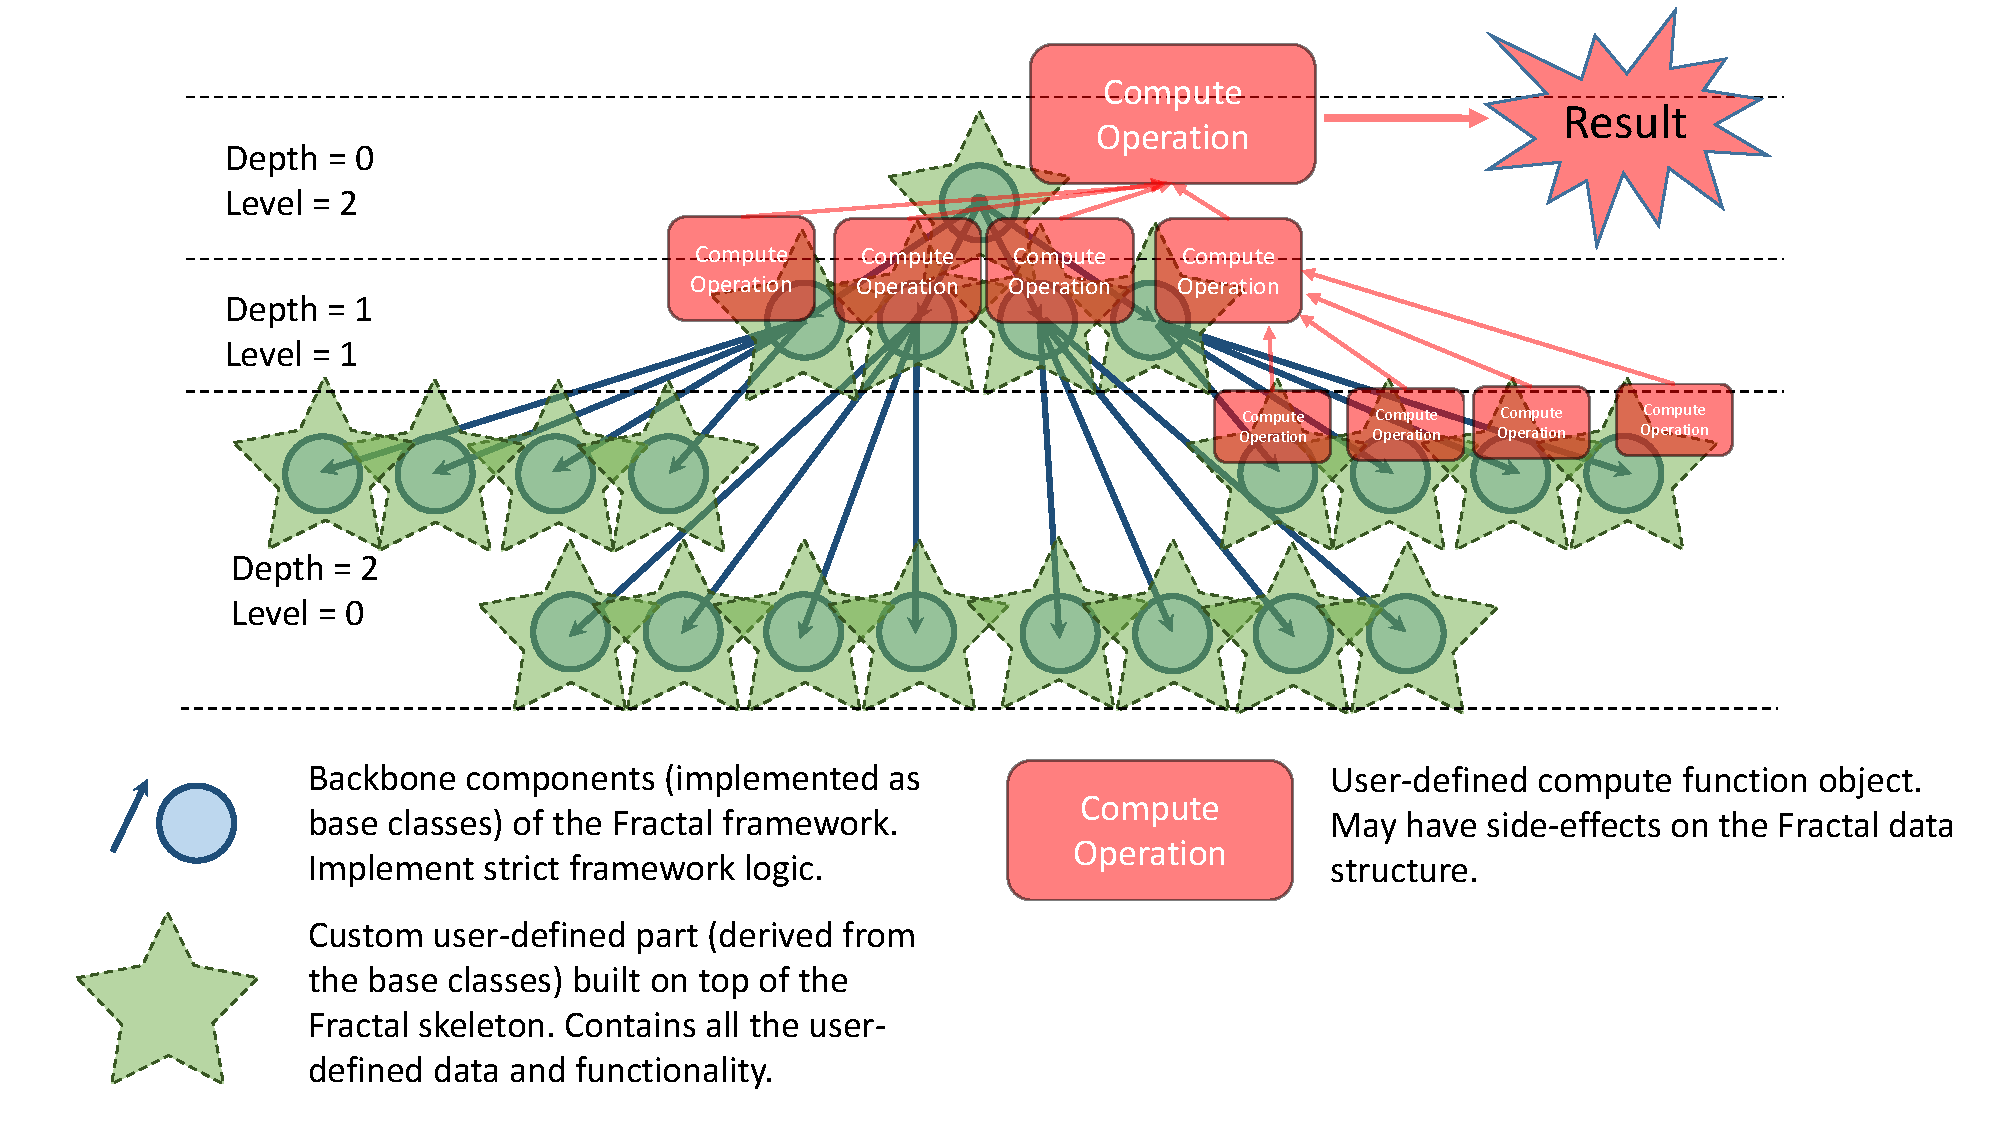
\includegraphics[width=1.0\textwidth]{images/Fractal.pdf}
\caption{The Fractal computational framework.}
\label{fig:fractal}
\end{figure}
\quad A more complicated and interesting fractal example would be a square being continuously and recursively divided into 4 equal sub-squares (southwest, northwest, southeast and northeast). The deep-growing structure is actually a 4-ary tree as well. Imagine one wants to compute the perimeter of some figure. One way to do it would be to map the figure on the square plane and then turn the plane into a grid by continuously splitting the square into 4 equal sub-parts (southwest, northwest, southeast, northeast) till we reach the granularity size of the grid. Then we paint all the grid elements located inside the figure shape as black and those outside of it as white. We iterate over the grid and detect all points of color flips and add the size of the grid elements to the final sum, which at the end is going to approximate the perimeter of the figure. That is roughly what the perimeter benchmark does.\newline\null
\quad In all its generality the fractal is a pattern, which can be characterized with self-similarity, repeatedness, structuredness, inherent parallelizability and the exact numeric values such as its depth and arity. All that naturally maps onto the C++ implementation as a class template we describe below.

\subsubsection{The implementation}
\quad Fractal is the key framework in our prototype library.


\subsection{Fold}
\label{computational_frameworks_fold}
\quad The Fold computational framework has been inspired by the computation done in the power benchmark. The fold is not a new concept and has found a wide application in many functional languages. The C++ language provides std::accumulate() function template as a component of its Standard Template Library, which performs a functional fold over a given data structure, but contrary to our computational framework does not allow any side-effects and modifications to the elements of the data structure. Moreover, our C++ class template library provides an alternative interface to a user with an extensible customization space.\newline\null
\begin{figure}[ht]
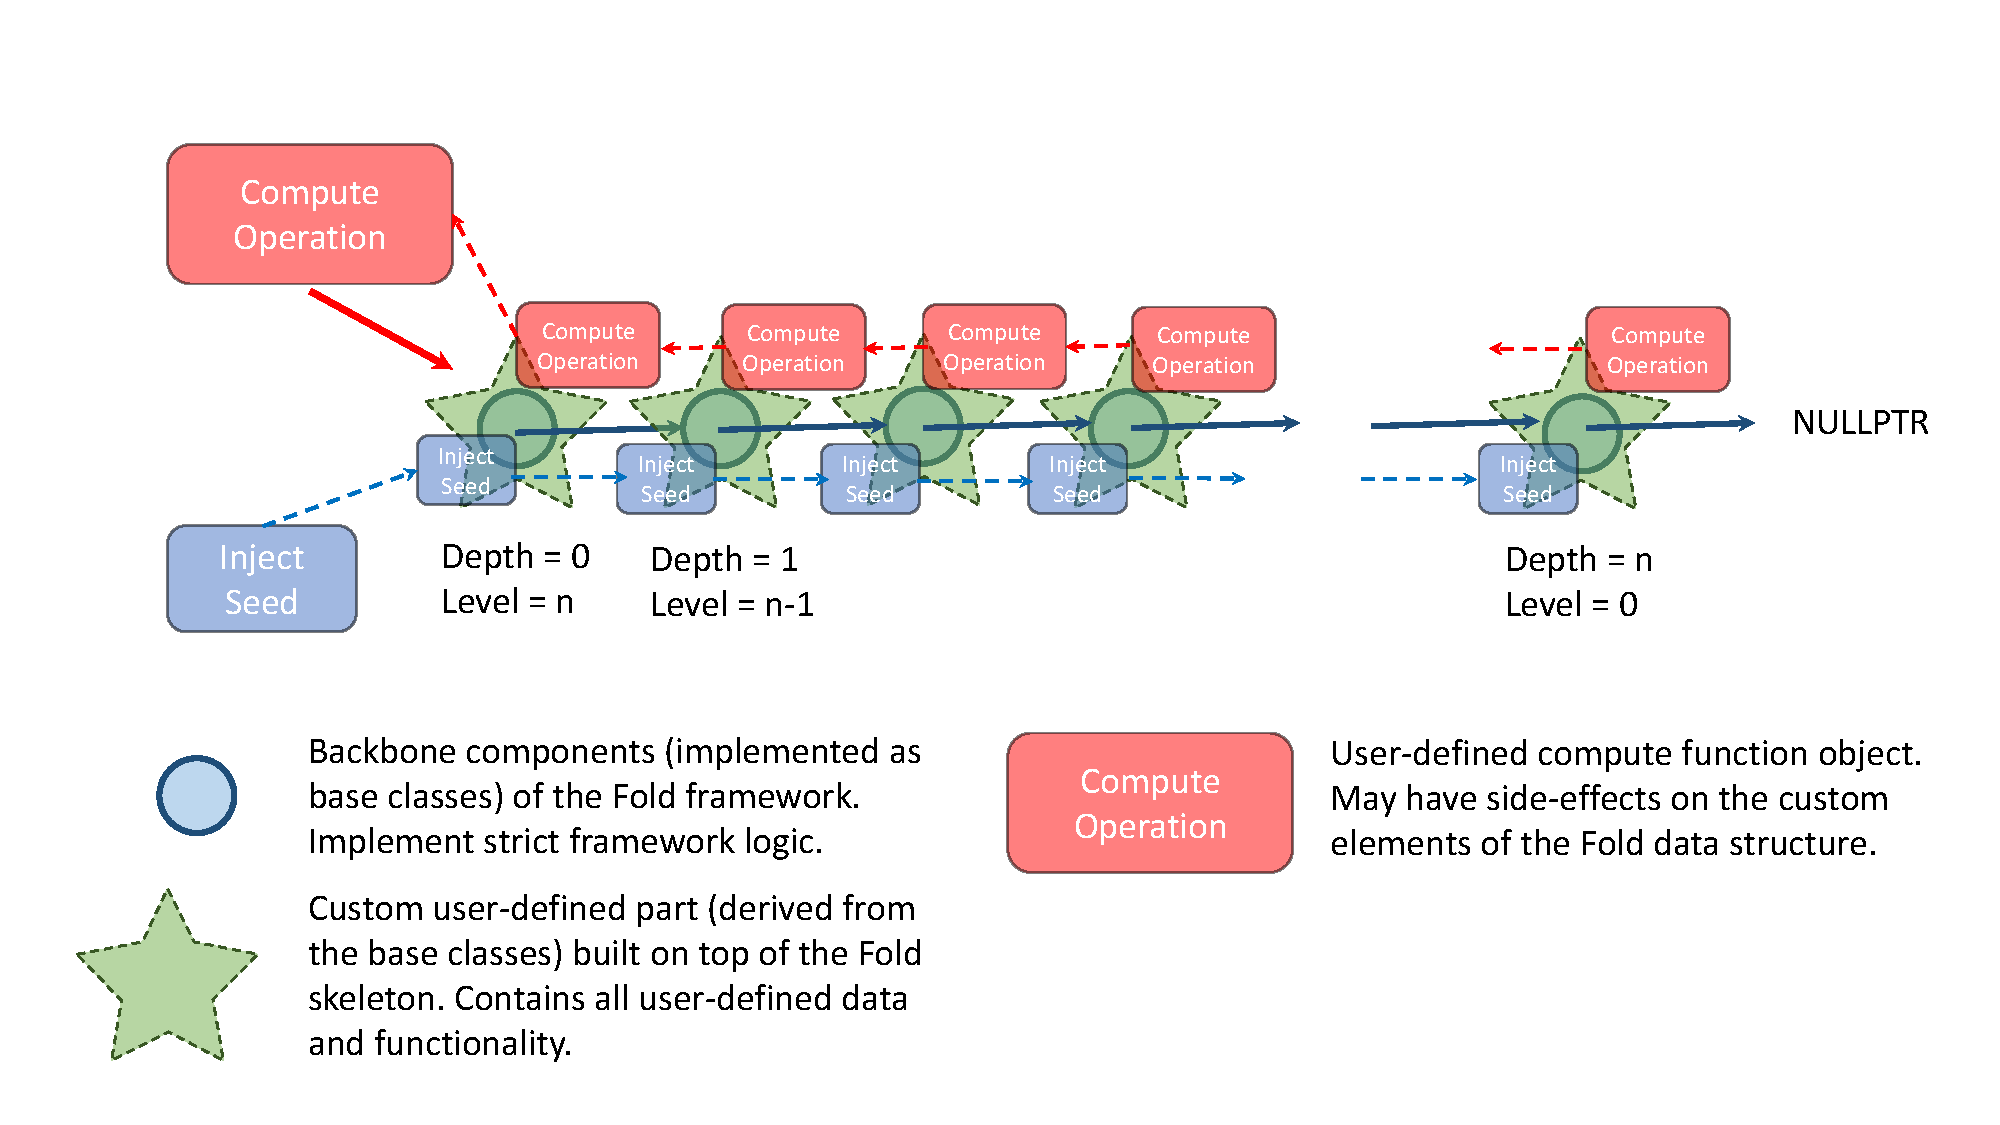
\includegraphics[width=1.0\textwidth]{images/Fold.pdf}
\caption{The Fold computational framework.}
\label{fig:fractal}
\end{figure}
\quad One can think of a Fold as a set of elements arranged into a linked-list. We grow the list to the specified depth given a seed value. Then we may inject some data into the head of the list and propagate it to its tail element. All propagation modifications are user-defined. Once every element of the list is ready with its data, the computation starts at the tail element and passes computed values back to previous elements of the chain.         


\subsection{Reduce}
\label{computational_frameworks_reduce}
\quad The Reduce computational framework is a well-known one. The difference between our computational framework and std::reduce() from C++ Standard Template Library (STL) is the possibility of having side effects and an alternative user customization interface. Our computational framework takes a function object with two overloaded and overridden virtual operator() methods. One specifies how to reduce the value from a single element (possibly changing the element in the process) and the other one defines the way of combining all the reduced values into the final return value. Our framework implements sequential as well as parallel Reduce versions.  


\subsection{Frameworks Library Design and Implementation}
\label{computational_frameworks_library_design}
\quad The design and implementation of computational frameworks library have been done iteratively using 4 Olden benchmarks as inspiration and  
The design of the C++ computational frameworks library aims at several goals.  
\begin{description}
\item[Modern C++] The implementation of the library is based on the Standard Template Library (STL) data structures, uses move semantics and unique pointers to achieve efficiency and smart memory management. For parallelization library uses OpenMP standard. All that provides for a wide source-code portability. The library is composed of a set of header files with class templates, which are supposed to be included into the user application.  
\item[Convenience] 
\item[Coherence] All computational frameworks in the library share the same user interface as well as internal design. Frameworks are inter-operable and flexible: one can create say, a fold of fractals of reductions. Different components can compute different return types.

\item[Sound design] CRTP, Algorithm Template pattern
\end{description}
\quad The computational frameworks are designed as a set of C++ class templates. The user interface these templates provide has been designed and refined iteratively using the set of Olden benchmarks [].     

\begin{minipage}[t]{\linewidth}
\begin{lstlisting}[caption={Computational framework class template skeleton},label={lst:framework_template_skeleton},language=C++]

template <typename ElemType, typename SeedType>
class Framework {
    public:
        class Element {
            // user-exposed customization iface
            virtual void grow(SeedType) = 0;
            virtual bool growth_stop_condition() { return false; }
        };
        template <typename ComputeType>
        class ComputeFunction {
            // framework specific application function API
            virtual operator()(ElemType& elem, ... ) = 0;
            virtual operator(const std::vector<ComputeType>&) = 0;
*       };
   /     
        void grow(size_t size, SeedType seed) {
            // organise framework elements 
            // into a data structure
            ... = new ElemType(); 
        }
        template<typename ComputeType>
        ComputeType compute(ComputeFunction<ComputeType>& apply_func);
    
    private:
        // framework data structure organisation
        // (list, tree, array, etc.)
};

\end{lstlisting}
\end{minipage}

\quad The design and the implementation of our template library reflect the target goals of the concept of computational frameworks.    

\quad There were several questions raised in the design process of a template library. 

\section{Performance study of the library}
\label{frameworks_performance_study}
\quad We have conducted a thorough examination of our prototype library. For that purpose we used 4 Olden benchmarks. Benchmarks \textit{health}, \textit{treeadd} and \textit{perimeter} fit into our \textbf{fractal} framework and stress it from different angles. We used the \textit{power} benchmark to test the practical operation of our \textbf{fold} and \textbf{reduce} frameworks.\newline\null
\quad We have rewritten original sequential legacy C implementations of the benchmarks with our prototype library in a modern, structured and well-designed way. The implementation can be configured to to be sequential or parallel. The fractal in the most general case is based on N-ary unbalanced tree.   


of 4 Olden benchmarks: health, perimeter, treeadd and power. The table below shows the performance gains our versions have over old sequential implementations.   

\section{Future work}
\label{frameworks_future_work}
\quad The concept of computational frameworks and the prototype library form the basis for the future work. We believe that the process of software parallelization with the help of computational frameworks can be further automated for a relatively simple applications (like Olden benchmarks). To back this feeling let's consider the health benchmark from the Olden suite. In particular, let's consider the grow() method, which allocates and grows the tree of villages.
\quad Listing \ref{lst:future_work_original} shows the original \textit{alloc\_tree()} function. It takes an integer argument \textit{level}, which specifies the depth of the tree to grow, then it takes an integer seed \textit{label} to initialize the element and a pointer \textit{back} to link the parent node to its children. In the body of the function we allocate dynamic memory for the node using \textit{malloc} call and call the \textit{alloc\_tree} function recursively in a loop of 4 iterations. The function returns a pointer to the created child subtree and the loop at the bottom of procedure links these pointers to a newly allocated and initialized node. For the initialization we calculate the number of personnel in a hospital and prepare the various lists of patients (waiting, inside, assessment, returned, etc.).\newline\null

\begin{minipage}[t]{\linewidth}
\begin{lstlisting}[caption={Computational framework class template skeleton},label={lst:future_work_original},language=C]

struct Village* alloc_tree(int level, int label, struct Village* back) {
    
    if (level == 0) {
        return NULL;
    } else {
        struct Village* new;
        int i;
        struct Village* fval[4];

        new = (struct Village*) malloc(sizeof(struct Village));

        for (i = 3; i >= 0; i--)
            fval[i] = alloc_tree(level-1, label*4+i+1, new, i);

        new->back = back;
        new->seed = label * (IQ + seed); 
        new->hosp.personnel = (int)pow(2, level - 1);
        new->hosp.assess.forward = NULL;
        new->hosp.assess.back = NULL;
        new->hosp.assess.patient = NULL;
        new->hosp.waiting.forward = NULL;
        ...
        new->returned.patient = NULL;

        for (i = 0; i < 4; i++)
            new->forward[i] = fval[i];

        return new;
    }
}

int main() {
    struct Village* top = alloc_tree(max_level, 0, top, 0);
}
\end{lstlisting}
\end{minipage}

\quad One can view the recursive creation of the tree with all its node linking and allocation operations as the \textbf{backbone logic}. On the contrary, the node initialization forms a custom part and can be viewed as the \textbf{business logic}. The backbone logic of the health benchmark corresponds to the fractal computational framework. The business logic should go into corresponding customization slots of the framework. So, the high level task is to identify what kind of a backbone logic (what kind of a computational framework) the code is doing, decouple the backbone part from a custom business logic and to insert the business logic into appropriate interfaces of the identified computational framework. Technically, for benchmarks as simple as Olden the technique can work on the level of compiler's front end: source code or an abstract syntax tree (AST). Health benchmark is simple. After we have identified the backbone logic to be that of a fractal, we can simply strip it off. Everything what's left is the business logic. The next step is to insert different parts of the business logic into the right API interfaces of the computational framework. 

\quad Listing \ref{lst:future_work_frameworks} shows what the final code should look like. Here we instantiate the fractal class template and fill its template methods with the extracted business logic. The next seed argument of the \textit{alloc\_tree()} function goes into the separate API slot of the framework, namely \textit{spawn\_child\_seed()}. The initialization of the village hospital goes into an overriden virtual \textit{grow()} method of the fractal element.

\begin{minipage}[t]{\linewidth}
\begin{lstlisting}[caption={Computational framework class template skeleton},label={lst:future_work_frameworks},language=C++]

void Village::grow(Fractal_t::Seed_t s) {
    if (this->element_info().level == 0) {
        return;
    } else {
        this->seed = s * (IQ + ::seed); 
        this->hosp.personnel = (int) pow(2, this->element_info().level-1);
        this->hosp.assess.forward = NULL;
        this->hosp.assess.back = NULL;
        this->hosp.assess.patient = NULL;
        this->hosp.waiting.forward = NULL;
        ...
        this->returned.patient = NULL;
        return;
    }
}

Fractal_t::Seed_t Village::spawn_child_seed(int child_id) {
    return (4*this->label+child_id+1);
}

bool Village::growth_stop_condition() {
    return false;
}

int main(int argc, char *argv[]) { 
    Fractal_t fractal;
    Fractal_t::Seed_t s = 0;
    fractal.grow(max_level-1, s);
}
\end{lstlisting}
\end{minipage}

\quad We need to fish out of the original code the actual type of the fractal element as well. Listing \ref{lst:future_work_element_original} shows the original definition of the \textit{Village} structure. Listing \ref{lst:future_work_element_frameworks} shows the target source code to be generated, where all data fields and customization parts are framed into the library API.

\begin{minipage}[t]{\linewidth}
\begin{lstlisting}[caption={Computational framework class template skeleton},label={lst:future_work_element_original},language=C]
struct Village {
    struct Village* forward[4];
    struct Village* back;
    struct List returned;
    struct Hosp hosp;   
    int label;
    long long seed;
};
\end{lstlisting}
\end{minipage}

\begin{minipage}[t]{\linewidth}
\begin{lstlisting}[caption={Computational framework class template skeleton},label={lst:future_work_element_frameworks},language=C++]
using Fractal_Element_t = class Village;
using Fractal_Seed_t = int;
const size_t Fractal_Arity = 4;
using Fractal_t = Fractal<Fractal_Element_t,Fractal_Seed_t,Fractal_Arity>;

class Village : public Fractal_t::Element {

    public:
        
        Village(Fractal_t::ElementInfo info) : Fractal_t::Element(info) {}
        ~Village() {}

        void grow(Fractal_t::Seed_t seed) override;
        Fractal_t::Seed_t spawn_child_seed(int child_id) override;

        struct List returned;
        struct Hosp hosp;
        int label;
        long long seed;
};
\end{lstlisting}
\end{minipage}

\quad For computation methods the process is alike to the one described above for growth methods. Figure \ref{fig:parallelization_scheme} illustrates the high level scheme of our approach. We call it an alternative parallelization scheme. Contrary to the 

\begin{figure}[ht]
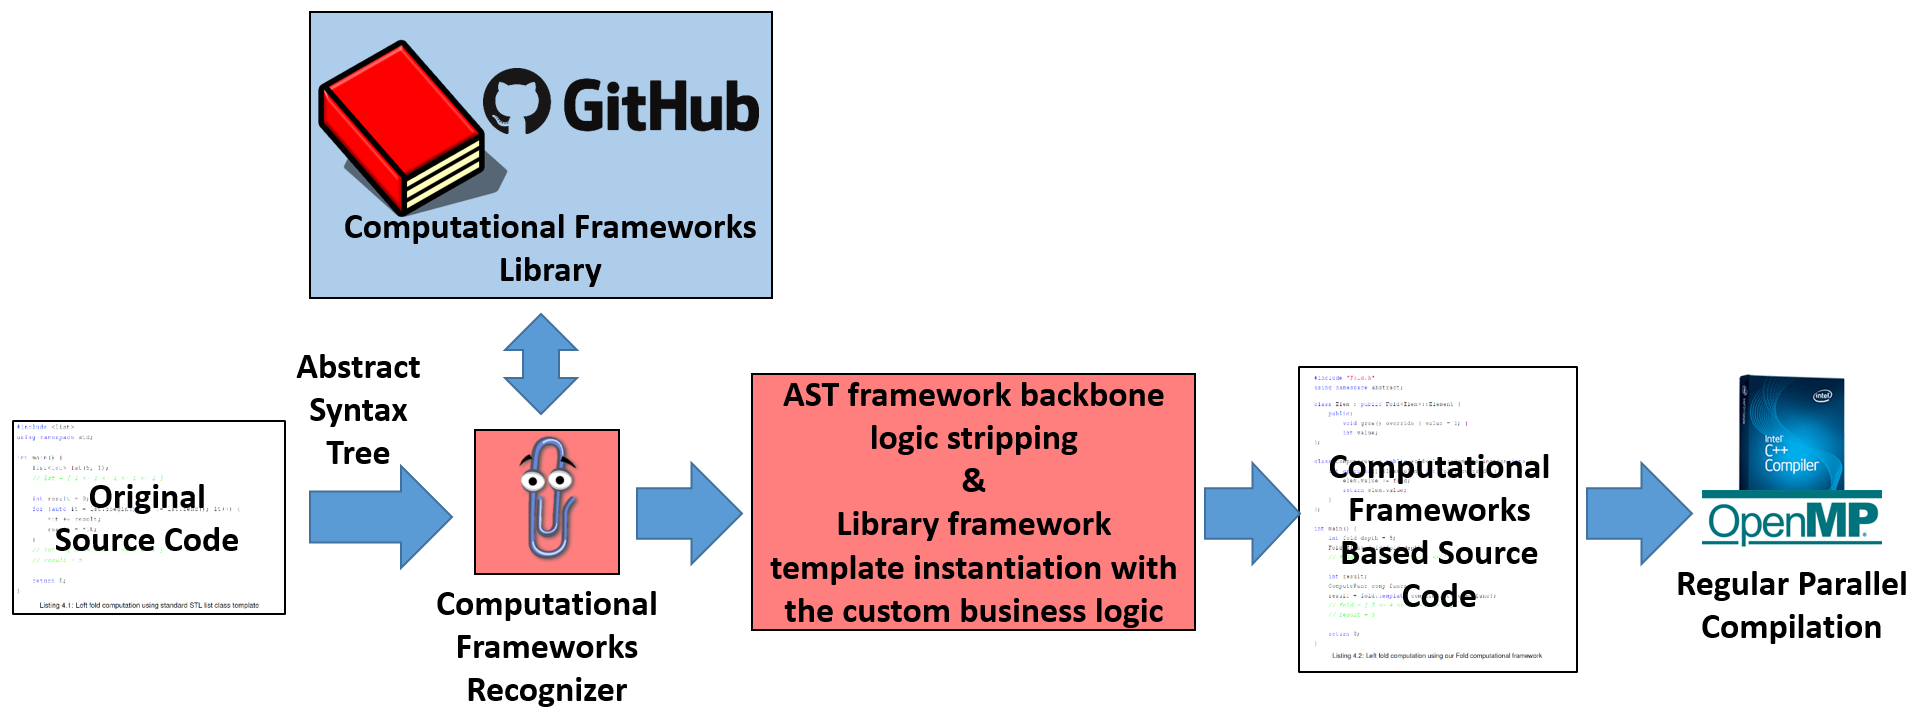
\includegraphics[width=1.0\textwidth]{images/parallelization_scheme.png}
\caption{An alternative software parallelization scheme. Works at the level of abstract syntax tree.}
\label{fig:parallelization_scheme}
\end{figure}

